In chapter \ref{ch1b}, we assumed that the wave field had spatially homogeneous amplitudes, propagating over a flat bottom. 
We will now allow the water depth to vary, which, like variations in the current velocity in chapter \ref{ch_current}, causes important 
wave modifications. 

\section{Wave shoaling}
In the absence of current, wave rays are orthogonal to wave crests are streamlines for the energy.
Considering two rays of the same monochromatic wave train, parallel in a
region where $C$ is uniform (for instance in deep water, $KD>>1$, and without
current) and spaced from $\Delta l$, the energy flux between those two rays
 $C_g E \Delta l$ is conserved along this 'tube'. All these properties can be
 demonstrated from Laplace equation and from the boundary conditions at the surface
 and at the bottom, assuming that amplitudes and phase velocities vary slowly.


Without current and for a beach with an uniform topography along the $y$-axis 
(longshore), wave propagation along the $x$-axis have therefore rectilinear
rays et $\Delta l$ does not change along the tube defined par two of its rays.
Hence, the spectral density of energy $E$ matches the group velocity $C_g$ changes
(see figure \ref{Cg}) so that the energy flux $C_g E$ remains constant.
In particular, in the coastal area, $C_g=\left(gD\right)^{1/2}$, therefore,
the spectral density of energy increases as $D^{-1/2}$. Yet, $E$ is proportional
to the mean or significant wave height squared $H_{\mathrm{rms}}=2^{-1/2} H_s$ and
$H_s=4 \left(E/\rho g\right)^{1/2}$. Therefore, the wave height increases as
$D^{-1/4}$. In practice the wave height is limited for wave breaking when  $D$ approaches zero. 

This modification of the wave height due to variations of the group velocity is called 
shoaling.  But on a real shoal, which has a finite length, the non-uniformity of the depth along the crests 
also causes refraction. 

\section{Refraction}

We showed in chapter \ref{ch1b} that the wave phase velocity was a
function of frequency and water depth. In presence of an horizontal current
${\mathbf U}({\mathbf x})$, vertically uniform, we observe a Doppler
shift as well. The wave angular frequency, in a fixed referential becomes
then, $\omega=\sigma+{\mathbf k}\bcdot{\mathbf U}$,  and the phase speed 
is :
\begin{equation}
    C=\frac{\omega}{k}
    = \left[ \frac{g}{k} \tanh \left(k D \right) \right]^{1/2}
    +\frac{1}{k}{\mathbf k}\bcdot{\mathbf U}
\end{equation}
The phase speed $C$ changes induce the refraction phenomenon, discovered
by Snel and Descartes in optics.


Without current, this effect is perceptible from the moment that
the water depth is less than half the wave length ($kD<\pi$).
Considering two areas with uniform water depths $D_1$ and
$D_2$ for $x<0$ and $x>0$, then the Snel law (also attributed to
Descartes\footnote{The Dutch mathematician Willebrord Snel discovered
the refraction law in 1621, but it was only published in 1703 in
Christian Huygens's book {\it Dioptrica} where Snel is named
in latin (Snellius) which leads to the frequent errors of the
English speakers that write his name Snell instead of Snel. The french
philosoph Ren{\'e} Descartes gives the Snel law in his treaty {\it La dioptrique},
an appendix of his famous {\it Discours de la m{\'e}thode pour bien conduire sa raison
et chercher la v{\'e}rit{\'e} dans les sciences} publish in Leiden in 1637
and apparently inspired from Snel's work, although Descartes repeated
Snel's experiments in 1626 and 1627.(Source: the
MacTutor history of mathematics archive, University of St Andrews,
Scotland, http://www-groups.dcs.st-andrews.ac.uk/{$\sim$}history)})
applies and expresses the wavenumber $k_y$ at the boundary,

\begin{equation}
    \frac{\sin \theta_1}{C_1}=\frac{\sin \theta_2}{C_2}
\end{equation}


Where $\theta_1$ et $\theta_2$ are the angles between the propagation
direction and the x-axis. This results applies to a beach with a topography
uniform along the y-axis. In this situation, $\sin \theta/C$ is conserved
by refraction  (figure \ref{fig:Snel}).

All the results of geometric optics apply, replacing light velocity by $C$,
in particular Fermat's principle: the integral of $C$ along a trajectory is
minimum in the variational sense. Hence, a bump at the bottom acts like a
optical converging lens while a trough will be divergent. This explains why
waves converge towards capes, increasing their height.
Waves propagating against a localized current vein (the current speed is zero
outside the current vein) are deviated toward its center. In addition to being shortened
due to the Doppler effect, waves are higher and steeper, hence more dangerous,
as in the Aguhlas current.

We can obtain a differential equation for the trajectories followed by waves from
that same principle. These trajectories are also called rays of characteristics.
Let $\left(x,y,\theta\right)$ be the position and direction of waves in a single
point of the ray, and $s$ the curvilinear coordinate along the ray, without current,

\begin{eqnarray}
\label{Ray eq}
\frac{\mathrm{d}x}{\mathrm{d}s} &=&\cos \left( \theta \right),  \label{Ray eq 1} \\
\frac{\mathrm{d}y}{\mathrm{d}s} &=&\sin \left( \theta \right),  \label{Ray eq 2} \\
\frac{\mathrm{d}\theta }{\mathrm{d}s} &=&\frac{1}{C}\frac{dC}{dh}\left[ \frac{dh}{dx}\cdot
\sin \left( \theta \right) -\frac{dh}{dy}\cdot \cos \left( \theta \right)
\right].  \label{Ray eq 3}
\end{eqnarray}

Without current, the motion of a wave packet is given by his speed
$\mathrm{d}s/\mathrm{d}t=C_g$ in the direction $\theta$.

%%%%%%%%%%%%%%%%%%%%%%%%%%%%%%%%%%%%%%%%%%%%%%%%%%%%%%% figure
\begin{figure}[htb]
\centerline{\includegraphics[width=0.7\textwidth]{FIGS_CH_SHALLOWLIN/refraction_Snel.pdf}}
    \caption{Propagation directions for incident or reflected waves, for each part of two
    phase speed $C$ discontinuities. For a natural topography, refraction is steady and the intensity
    of reflected waves is generally weak.}
\label{fig:Snel}
\end{figure}
%%%%%%%%%%%%%%%%%%%%%%%%%%%%%%%%%%%%%%%%%%%%%% end of figure

%%%%%%%%%%%%%%%%%%%%%%%%%%%%%%%%%%%%%%%%%%%%%%%%%%%%%%% figure
\begin{figure}
\centerline{\includegraphics[width=0.8\textwidth]{FIGS_CH_SHALLOWLIN/Long_Beach.pdf}}
  \caption{Refraction diagram for waves of 20~s period from 160$^\circ$ at Long Beach harbor, California}{From \cite{Lacombe1950}. 
  Note the units on the dashed depth contours: 1 fathom is 1.83~m.  }
   \label{RaysLongBeach}
  \end{figure}
%%%%%%%%%%%%%%%%%%%%%%%%%%%%%%%%%%%%%%%%%%%%%%%%%%%%%%% figure

%%%%%%%%%%%%%%%%%%%%%%%%%%%%%%%%%%%%%%%%%%%%%%%%%%%%%%% figure
\begin{figure}
\centerline{\includegraphics[width=0.8\textwidth]{FIGS_CH_SHALLOWLIN/Cap_Breton.png}}
  \caption{Refraction diagram for 12~s swell over the Gouf de Cap Breton}{From \cite{Lacombe1950}.}  
   \label{RaysCapBreton}
  \end{figure}
%%%%%%%%%%%%%%%%%%%%%%%%%%%%%%%%%%%%%%%%%%%%%%%%%%%%%%% figure

%%%%%%%%%%%%%%%%%%%%%%%%%%%%%%%%%%%%%%%%%%%%%%%%%%%%%%% figure
\begin{figure}
\centerline{\includegraphics[width=0.63\textwidth]{FIGS_CH_SHALLOWLIN/NCEX_rays.png}}
  
    \caption{Examples of two wave rays methods}{a. "Traditional" computation for a west swell with a 15-s period,
    near La Jolla, California. The location of some the wave buoys deployed during the NCEX experiment is indicated
    by numbers 32 to 37 and the  10, 50, 100 et 200~m isobaths are shown by the dashed lines. From Magne et al. 
    (2007\nocite{Magne&al.2007}). b. computation of back-trajectories from point 34, for the same 
    period $T=15~s$ and arrival directions evenly spaced with a 1$^\circ$ interval. Only the wave rays reaching
    offshore, and able to bring energy at point 34 are shown (this is true only within the optical geometry approximation,
    and by neglecting the wave reflection at the shore. Regular marks are visible along the ray and correspond to
    the distance covered by the group velocity within time intervals of 60 seconds.)}
  
   \label{RaysLaJolla}
  \end{figure}
%%%%%%%%%%%%%%%%%%%%%%%%%%%%%%%%%%%%%%%%%%%%%%%%%%%%%%% figure

With a current $\mathrm{d}s/\mathrm{d}t=\left|{\mathbf C}_g+{\mathbf
U}\right|$ and the wave propagation direction is different from the direction
perpendicular to wave crests. These "rays" have long been calculated by hand
\citep{Munk&Traylor1947} before numerical methods took over \cite{Dobson1967}.
 
 It is very insightful to look at wave plans, the diagrams showing the ray spacing from directions parallel offshore. (see example in figure
 \ref{RaysLongBeach}). From the energy flux conservation between two rays, a ray spacing $l$ narrower than the offshore spacing $l_0$ means 
 that the local wave height increases. This is the case in front of Long Beach pier
 for the 20~s south swell. This augmentation only due to refraction, is of a factor $\sqrt{l_0/l}$,
 than needs to be multiplied by the shoaling coefficient $\sqrt{C_{g0}/C_g}$. This combination gives a seven-fold increase in wave height that explains the destruction of the Long Beach Pier
in April 1930 due to an unusual south swell \citep{Lacombe1950}. Indeed, only the very long swells can be refracted by the bottom topography at 200~m depth.
The pier has been rebuilt since its destruction but with a slightly different configuration.
This computation for Long Beach can be compared to the one for 12-s waves at Cap Breton, France (figure \ref{RaysCapBreton}). 

 When using a numerical calculation, back-trajectories from a fixed point are more reliable 
 (see for instance in figure \ref{RaysLaJolla}.b). That latter method avoids the occurrence of singularities such as 
 caustics that occur when forward-propagated rays cross. Indeed, geometrical optics predicts that the energy of a monochromatic wave train becomes infinite at the caustic. In fact, even under geometrical optics the 
wave height remains finite because rela waves are not monochromatic and the the caustics wave rays of the different spectral components are not at the same location. In the case of for monochromatic wave, the wave height is \textit{in fine} limited by wave breaking
or diffraction.  

When using backward ray tracing, we use the equality of the
 of the spectral densities in the coordinates $(k_x,k_y)$, between two points $A$ et $B$ 
 of the same ray. Hence for a zero source term, and in the stationary case without current, 
 using (\ref{eq:Eftheta_Ekxky}), equation (\ref{EulerianEBEdeep}) gives
 \begin{equation}
 E_A(f,\theta_A)=E_B(f,\theta_B)\frac{C_{g,B} k_A}{C_{g,A} k_B}\label{eq:ray_model},
\end{equation}
where $\theta_A$ et $\theta_B$ the ray directions when they cross $A$ and $B$, respectively.
One may hence transform an offshore spectrum to the coast to account for refraction and shoaling.
In this situation, we shall often assume that the offshore  spectrum is relatively uniform. 
Reciprocally, we may also estimate an offshore sea state from coastal measurements.
This technique can easily be extended to non-stationary situations by adding a time shift between
$A$ and $B$ corresponding to the propagation duration, i.e., the integral of $1/C_g$ along the ray.
The difficulty of these calculations are limited to the ray tracing that can be done once for all 
for stationary media (when the tide effect is negligible). This transformation method of a sea state
from offshore to the coastline is often very precise, especially for situations dominated by shoaling
and refraction \citep{OReilly&Guza1993,Ardhuin&al.2003a,Ardhuin2006a,Magne&al.2007}.





\section{Diffraction}
So far, we have considered that the wave amplitude and the properties of the medium in which they
propagate vary slowly in comparison to the wave period on wave length (WKB approximation).
%%%%%%%%%%%%%%%%%%%%%%%%%%%%%%%%%%%%%%%%%%%%%%%%%%%%%%% figure
\begin{figure}
\centerline{\includegraphics[width=0.4\textwidth]{FIGS_CH_SHALLOWLIN/NTUA_NCEX_en.png}}
  \caption{Example of propagation of a monochromatic 16~s period, 1~m amplitude offshore swell.}
  {Computation made with the finite differences elliptical extended Berkhoff model, from Athanassoulis et Belibassakis
  (1999)}
   \label{NTUA_NCEX}
  \end{figure}
%%%%%%%%%%%%%%%%%%%%%%%%%%%%%%%%%%%%%%%%%%%%%%%%%%%%%%% figure

It has been noticed earlier that for caustics due to refraction 
of a monochromatic wave, this WKB approximation is not valid. This assumption
is not verified in the vicinity of obstacles such as breakwaters.
For small amplitude waves, neglecting the wind effect and the bottom friction,
one may use the linearized equations. Over a flat bottom and with such obstacles,
a solution for $\phi$ can be found with the following equation
\begin{equation}
    \phi=\hat{\phi}({\mathbf x})\frac{\cosh\left(k_0 z+k_0 D\right)}{\cosh\left(k_0 D\right)}
     \mathrm{e}^{-\mathrm{i}\omega t}\quad +\quad \mbox{c. c.},
\end{equation}
where $\omega^2=gk_0 \tanh\left(k_0 D\right)$. $\phi$ verifies the cinematic
boundary conditions at the bottom and surface. The Laplace equation, simplifies
into the Helmoltz equation,
\begin{equation}
    \nabla^2 \hat{\phi}+k^2 \hat{\phi}=0.
\end{equation}

In general, the elliptic nature of that equation imposes a solution method
with boundary conditions specified along a closed contour. 

We can look at different approximations of the wave equation by taking a wave train with amplitude $\hat{\Phi}$ that varies slowly 
on the scale $\widetilde{\mathbf
x}=\varepsilon x$, giving a complex amplitude $\hat{\phi}=\hat{\Phi}\left(\widetilde{\mathbf
x}\right)\mathrm{e}^{\mathrm{i}S\left({\mathbf x}\right)}$, with a local wavenumber  ${\mathbf k}=\bnabla S$, 
that also varies slowly.  

Using that form in the Laplace equation gives
\begin{eqnarray}
    \nabla^2 \hat{\phi} & = & \bnabla \bcdot
    \left(\bnabla \hat{\Phi}\mathrm{e}^{\mathrm{i}S}\right)\\
    & = & \bnabla \bcdot \left[
    \left( \varepsilon \bnabla \hat{\Phi} + i{\mathbf k}\hat{\Phi}\right)
    \mathrm{e}^{\mathrm{i}S} \right]\\
    & = &  \left[\varepsilon^2 \nabla^2 \hat{\Phi}
    + 2\mathrm{i} \varepsilon {\mathbf k}\bcdot \bnabla \hat{\Phi}
    +\left(\mathrm{i} \varepsilon \bnabla \bcdot {\mathbf k}-k^2\right)\hat{\Phi}
     \right]\mathrm{e}^{\mathrm{i}S}\\
\end{eqnarray}

At zero order in $\varepsilon$, the variations of the amplitude
$\hat{\Phi}$ are neglected to keep only the phase variations,  $S\left({\mathbf x}\right)$,
and we obtain $\left|k\right|=k_0$ meaning that  wave trains propagate exactly like plane waves.

At first order, we neglect the spatial derivatives of  $\hat{\Phi}$.
One may show (Mei, 1989, chapter 3, see also Ardhuin et Herbers 2002\nocite{Ardhuin&Herbers2002})
that if the bottom slope is of order  $\varepsilon$ as well, other terms, in
addition to $\hat{\phi}$ are required to satisfy the kinematic boundary condition
at the surface and we get the action conservation equation,
\begin{equation}
    \frac{\partial}{\partial t} \left( \frac{E}{\sigma} \right)
    +\bnabla \bcdot \left( \frac{E}{\sigma} {\mathbf C}_g \right)=0.
\end{equation}

Diffraction appears with the second-order terms, and waves tend 
to turn towards regions with lowest wave amplitudes.

\cite{Berkhoff1972} used the approximation, now known as the mild slope approximation, 
that $\phi$  verifies the polarization and dispersion
relations of linear waves over a flat bottom. After some calculations, we obtain (see for instance Mei, 1989, chapter 3)
the so-called mild-slope equation (or Berkhoff's equation).
\begin{equation}
    \bnabla \bcdot \left( C C_g \bnabla \zeta\right) +\omega^2\frac{C_g}{C}\zeta=0.\label{eq:mild_slope}
\end{equation}

The mild slope equation (\ref{eq:mild_slope}) is an extension of the Helmoltz equation to a mild bottom slope. This equation 
is widely used in coastal engineering for determining harbor agitation, using
finite elements numerical models. Results of this type of model are shown in figure \ref{NTUA_NCEX}.

\cite{Radder1979} proposed a parabolic approximation
of the elliptic equation, by neglecting the $\zeta$ gradients in the
propagation direction, which conserves the diffraction effects. Such a
model (called refraction-diffraction model) has been used for swell forecasting
over the Californian Coastline (http://cdip.ucsd.edu), from offshore
prediction. The Californian continental shelf is indeed narrow enough to neglected
the local generation of waves.

However, contrary to what happens in the vicinity of coastal structures, 
the diffraction can generally be neglected in this region \cite{OReilly&Guza1991,Peak2004}. For example, during the
3-month long Near Canyon EXperiment (NCEX) offshore La Jolla, California, 
only one swell had been measured with a frequency low enough
to justify the use of a model solving Berkhoff's equation. In this situation the
Berkhoff's model provided slightly more accurate results than the ray tracing
method and only at a limited number of locations. These are the locations 
where the wave field varies strongly at the scale of the wavelength, with a variation
of a factor 5 in the wave amplitude across the Scripps canyon wall, over a distance shorter that the wavelength
(figure \ref{NCEXcomp}).


\begin{figure}
\centerline{\includegraphics[width=0.5\textwidth]{FIGS_CH_SHALLOWLIN/comparison_at_all_sites.pdf}}
  \caption{Wave observations and modeling during NCEX.}
  {The significant wave heights ($H_s$) for the frequency band 
   0.04-0.08~Hz are computed from the spectra measured from 1:30 to
   4:30 pm UTC, on November 30 2003. The buoy location are shown on figure
   \ref{RaysLaJolla}. The models used are: a ray back-tracing ("refraction", O'Reilly \& Guza 1991) 
   three elliptical models and a parabolic approximation of the Berkhoff equation
   ("Ref-dif" Kirby 1986\nocite{Kirby1986c}). The three models use the same numerical
   code and solve Berkhoff's equations ("Mild Slope Equation" or MSE,
  1972\nocite{Berkhoff1972}), their version modified by Massel  (MMSE,
  1993\nocite{Massel1993}) and their extension by the coupling of three evanescent modes and a local mode
  (NTUA5, Athanassoulis et Belibassakis 1999\nocite{Athanassoulis&Belibassakis1999}).
  The difference that appears between the refraction model and the elliptical models 
  at buoys 32, 36 and 37 is related to the wave transmission by tunnel effect across the canyon,
  despite its large depth (see also Thomson et al. 2005\nocite{Thomson&al.2005}). This tunnel effect
  can not be represented in the geometric optics approximation over which relies the ray tracing of the
  refraction model. Figure from \cite{Magne&al.2007}.}
 \label{NCEXcomp}
  \end{figure}

One may often just use the refraction computation given by eq. (\ref{eq:ray_model}).
This kind of approach take into account the details of the bathymetry
and of the spectral shape, which is very important form complex
coastline.

\section{Reflection}
Any variations of the water depth or current velocity - the wave guide parameters - result in partial reflections. These reflections are significant
only if the above cited variations are large over the wave length scale. This is the case when the waves approach the coastline.

\subsection{Reflection at the shoreline}
Hence, the magnitude of the reflection, that can be characterized by the ratio $R=a_r/a_i$ of the reflected and incident wave amplitudes, increases
strongly with the bottom slope $\beta$ and with the wave period $T$. 
%%%%%%%%%%%%% figure
\begin{figure}[htb]
\centerline{\includegraphics[width=0.5\textwidth]{FIGS_CH_SHALLOWLIN/R2_vs_Miche.png}}
  \caption{Energy Reflection coefficient $R^2$ as a function of the Miche number $M$, From Elgar et al. (1994), copyright American Meteorological Society.}
\label{fig:Miche_ref}
\end{figure}
%%%%%%%%%%%%% end of figure
\cite{Miche1951} studied monochromatic waves over a constant bottom slope
and reported that $R^2$ is roughly equal to the coefficient
\begin{equation}
M=\frac{0.0016 g^2 \tan^5 \beta  T^4}{H_{\infty}^2},
\end{equation}
where  $H_{\infty}$ is the offshore wave height, in the case $M < 1$ and $R=1$ for $M > 1$. 
The only precise study published on the topic of in situ random waves shows that, using $H_s$ instead of $H$, Miche parameter $M$
effectively gives an order of magnitude of the reflection coefficient for swells and wind seas (figure \ref{fig:Miche_ref}). 


The study of \cite{Elgar&al.1994} suggests that $R^2 > M$ for $M<0.05$ and $R^2 < M$ for $M>0.1$.
A better approximation, $R^2=\min\{0.007(\log_{10}(M)+5)+0.2 M,1\}$, has been implemented by \cite{Ardhuin&Roland2012} in the WAVEWATCH III model.
Besides, for a given sea state, the reflection decreases toward high frequencies. 

Casual observation of wave reflection from a beach suggests that, in addition to the reflection there is also a generation of short wave components, that 
are radiated toward the open ocean. To our knowledge, this has not yet been discussed in scientific publications. 


\subsection{Reflection by underwater topography}

The variations $h'$ of the water depth at the wave length scale also impact waves.
One way to represent this effect in the spectral evolution equation consists in
decomposing the topography variation $h'$ in sine waves of wavenumber $l$,
\begin{equation}
h'\left({\mathbf x}\right) =\sum_{{\mathbf l}}
B_{{\mathbf l}}\left( \widetilde{\mathbf x}\right)
\mathrm{e}^{\mathrm{i}{\mathbf l}\bcdot{\mathbf x}},  \label{h}
\end{equation}
and to calculate the interaction of the wave spectrum with each sine wave.
Strictly speaking, we obtain a wave forcing by the topography. % as obtained in Chapter 2 for the wind turbulence (Hasselmann, 1966\nocite{Hasselmann1966}).
At fist order in bottom slope ($\varepsilon = lh$), we obtain a resonance between
two waves with wave numbers ${\mathbf k}$ et ${\mathbf k}^{\prime }$, such as
$k=k^\prime$, that exchange energy thanks to bottom ripples with wave number
${\mathbf l}={\mathbf k}-{\mathbf k}^{\prime}$. This leads to an energy transfer
in other directions (figure \ref{fig:Braggscattering2}).


%%%%%%%%%%%%% figure
\begin{figure}[htb]
\centerline{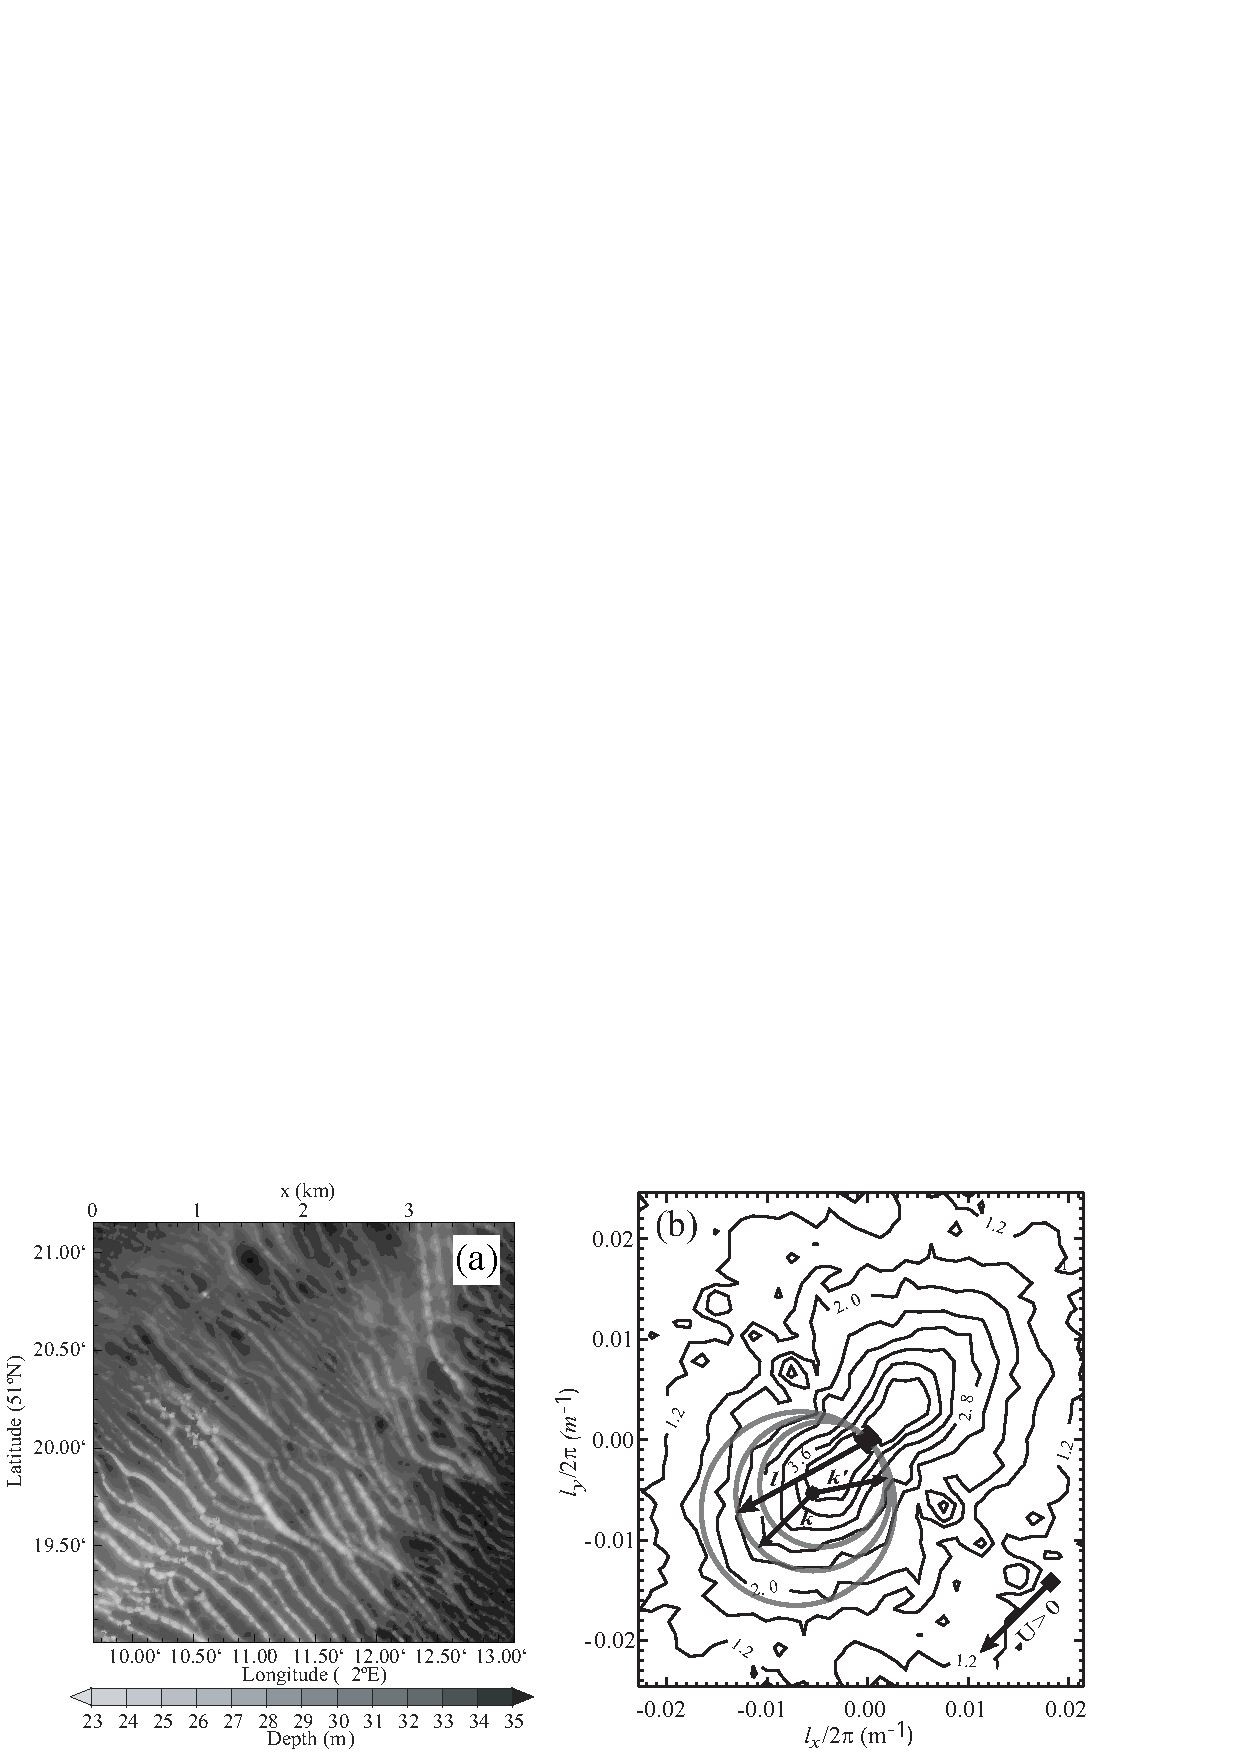
\includegraphics[width=\textwidth]{FIGS_CH_SHALLOWLIN/figure_whitepaper72.jpg}}
  \caption{Bathymetry of a region with underwater dunes in the south of the North Sea.}{On the
  spectrum (b) of this bathymetry, the contours indicate the value  $log_{10}[4\pi F_B({\mathbf l})]$
  with F$_B$ the bottom spectrum. The circles indicate the components ${\mathbf l}$ that interact
  with waves of 12.5~s period coming from the North-West (wave number ${\mathbf k}$) for 3 current
  speeds, -2, 0 et 2~m/s. .}\label{fig:Braggscattering1}
\end{figure}
%%%%%%%%%%%%% end of figure

%%%%%%%%%%%%% figure
\begin{figure}[htb]
\centerline{\includegraphics[width=0.8\textwidth]{FIGS_CH_SHALLOWLIN/figure_whitepaper73.jpg}}
  \caption{Example of spectral evolution caused by bottom reflection for the wave spectrum shown in 
  figure \ref{fig:Braggscattering1} and applied in 20~m depth }{(a) computation domain, (b) incident spectrum imposed at point F,
  (c) and (d) evolution term of the spectrum with and without current, (e) spectrum at point O, 40 km inside the domain after
  5 hours of propagation. The frequency is here the relative frequency $\sigma/(2 \pi)$.}\label{fig:Braggscattering2}
\end{figure}
%%%%%%%%%%%%% end of figure

The local effect of this Bragg diffusion is a modification of the
directional wave spectrum. If the bottom topography is dominated
by large scales ($l<< k$), the result is an increase of the waves directional
spreading, that corresponds to a shortening of the wave crest length,
rendering the wave field appearance messier.

For a topography with a large spectral density at $l=2k$, the wave
are back-scattered \citep{Heathershaw1982}
and the wave height decreases in the initial direction of wave 
propagation. For random waves this effect takes the form of 
 a bottom induced scattering term  $S_{\mathrm{bscat}}$ \citep{Ardhuin&Magne2007}, which typically 
 produces a broadening of the directional spectrum when important depth variations are present at the scale 
 of the wavelength.

\subsection{Summary}
In Shallow water ($D <0,5 L$), waves are influenced by the bottom in addition
to wave-wave interaction and interaction with atmosphere. Leaving apart wave breaking
that occurs in the direct vicinity of the beach, the bottom effect depends on the 
relative amplitude of the waves and of the bottom topography. All these effects
are supposed independent of each other, and independent of the wave-wave interaction
or of the interaction between waves and atmosphere \citep[e.g.][]{WAMBook}. 
This leads to a spectral evolution equation that takes
into account all the processes as source terms. This is thus an extension of 
the deep-water action balance given by eq. (\ref{Action_balance}) with additional source terms, 
\begin{equation}
S=S_{\mathrm{in}}+S_{\mathrm{nl}}+S_{\mathrm{dis}}+S_{\mathrm{fric}}
    +S_{\mathrm{bscat}}+ \cdot \cdot \cdot
\end{equation}

